
%%%%%%%%%%%%%%%%%%%%%%%%%%%%%%%%%%%%%%%%%%%%%%%%%%%%%%%%%%%%%%%%%%%%%%%
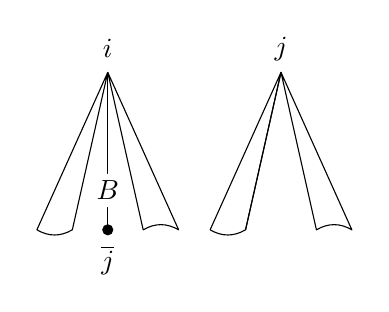
\begin{tikzpicture}[
edge from parent path=,
level distance=2cm,
level 1/.style={sibling distance=0.45cm}
%,scale=1, every node/.style={transform shape}
]

  \tikzstyle{ref}=[circle,fill=black,inner sep=0.5mm]
%  \tikzstyle{ref2}=[circle,fill=black!40,inner sep=0.5mm]
  \tikzstyle{dashdot}=[dashed,dash pattern=on 2pt off 1pt on 0.5pt off 1pt]
  \tikzstyle{mysnake}=[decorate,decoration={snake,amplitude=0.3mm,segment length=0.75cm}]

  \node (c1) {}
    child { node (c11) {} }
    child { node (c12) {} }
    child { node (c13) [ref,label={below:$\overline{j}$}] {} }
    child { node (c14) {} }
    child { node (c15) {} };

  \node (c10) [minimum height=0.5cm,node distance=0.3cm,above of=c1] {$i$};

  \draw [join=round] (c1.center)
    to (c11.center)
    to [bend right] (c12.center)
    -- cycle;

%  \draw [join=round] (c12.center)
%    to [bend right](c13.center) 
%    to [bend left] (c14.center)
%    to (c1.center);

  \draw (c1.center) to node [near end,circle,fill=white,inner sep=0.5pt] {$B$} (c13.center);

  \draw [join=round] (c1.center)
	to (c14.center)
    to [bend left] (c15.center)
    to (c1.center);

%  \begin{pgfonlayer}{background}
%  \path [left color=white,right color=black!40,shading=axis] (c12.center)
%    to [bend right] (c13.center)
%    to [bend left] (c14.center)
%    to (c1.center);
%  \draw [mysnake,dashdot] (c1.center) -- (c13.center);
%  \end{pgfonlayer}


  \node (c2) [node distance=2.2cm,right of=c1] {}
    child { node (c22) {} }
    child { node (c23) {} }
%    child { node (c24) [ref,label={below:$\overline{i}$}] {} }
    child { node (c24) {} }
    child { node (c25) {} }
    child { node (c26) {} };

  \node (c20) [minimum height=0.5cm,node distance=0.3cm,above of=c2] {$j$};

  \draw [join=round] (c2.center) -- (c23.center);

  \draw [join=round] (c2.center)
    to (c22.center) 
    to [bend right] (c23.center)
    -- cycle;

%  \draw [join=round] (c23.center)
%	to [bend left] (c24.center)
%    to [bend right] (c25.center)
%    to (c2.center);

  \draw [join=round] (c25.center)
    to [bend left] (c26.center) 
    to (c2.center) -- cycle;

%  \begin{pgfonlayer}{background}
%  \path [left color=white,right color=black!40,shading=axis] (c23.center)
%    to [bend left] (c24.center)
%    to [bend right] (c25.center)
%    to (c2.center);
%  \draw [mysnake,dashdot] (c2.center) -- (c24.center);
%  \end{pgfonlayer}

\end{tikzpicture}
